\section{\texorpdfstring{$\mathbb{R}$ e la cardinalità del continuo}{R e la cardinalità del continuo}}

In questa sezione daremo una definizione di $\RR$ come insieme ordinato. Estenderemo, poi, la definizione ad includere le operazioni di campo, ma senza svolgere le verifiche.

\begin{definition}[Maggiorante, insieme superiormente limitato ed estremo superiore]
	Sia $(A,<)$ un ordine totale, allora:
	\begin{itemize}
		\item $m \in A$ è un \vocab{maggiorante} di $B \subseteq A$ se $\forall x \in B \; x \leq m$
		\item $B \subseteq A$ è \vocab{superiormente limitato} se ha un maggiorante
		\item $s\in A$ è \vocab{l'estremo superiore} di $B$ - denotato con $\sup B$ - se $s$ è il minimo dei maggioranti di $B$.
	\end{itemize}
\end{definition}

\begin{note}
	Non sempre gli estremi superiori esistono, e, se $B$ ha un estremo superiore, questo è unico\footnote{Segue dall'unicità del minimo di un insieme ordinato.}.
\end{note}

\begin{definition}[Ordine totale completo]
	Un ordine totale $(A,<)$ è \vocab{completo} se ogni $B \subseteq A$ superiormente limitato ha un estremo superiore $\sup B \in A$.\footnote{Questa per la precisione è la definizione di \vocab{Dedekind-completezza}.}.
\end{definition}

\begin{exercise}[$\QQ$ non è completo]
	\label{q_noncompleto}
	Dimostra, usando solo le proprietà di $\QQ$, che l'insieme $\{x \in \QQ | x^2 < 2\}$ non ha estremo superiore in $\QQ$.
\end{exercise}

\begin{lemma}[$\QQ$ è archimedeo]
	Diciamo che un campo ordinato $K$ soddisfa la \vocab{proprietà archimedea} se, dati $x,y \in F$, con $0 < x < y$, esiste $n \in \NN$ tale che $nx > y$.\footnote{O equivalentemente dato $x \in K$, con $x > 0$, esiste $n \in \NN$ tale che $n > x$.}
	$(\QQ,0,1,+,\cdot,\leq)$ è un campo ordinato archimedeo.
\end{lemma}

\begin{soln}
	
\end{soln}

In conseguenza dell'esercizio, possiamo dire che $\QQ$ non è completo. Costruiamo ora un ordine completo $(\RR,<)$ che contiene una copia isomorfa di $\QQ$ come sottoinsieme denso.

\begin{definition}[Segmento iniziale]
	Sia $(A,<)$ un ordine totale. $B \subseteq A$ è un \vocab{segmento iniziale} di $A$ se $\forall x \in B \; \forall y \in A \; y < x \rightarrow y \in B$ \textcolor{MidnightBlue}{- cioè se contiene un punto, contiene tutti i precedenti, strettamente}.
\end{definition}

Ossia $B$ è un segmento iniziale di $A$ se, ogniqualvolta $B$ contiene un elemento, $B$ contiene altresì tutti gli elementi minori di questo.
Un segmento iniziale $B$ di $A$ si dice \vocab{proprio} se $B \ne A$.

\begin{example}[Segmento iniziale principale]
	Dato $(A,<)$ ordine totale, $A$ stesso e $\emptyset$ sono segmenti iniziali di $A$. Dato $x \in A$, l'insieme:
	\[ A_x \Mydef \{y \in A | y < x\}
		\]
	è un segmento iniziale proprio di di $A$ - detto \vocab{segmento inziale principale} determinato da $x$. Ad esempio $\{x \in \QQ | x < 0 \lor x^2 < 2\}$
	è un segmento iniziale - proprio - di $\QQ$ che non è principale.
\end{example}

\begin{note}
	Useremo nuovamente il concetto di segmento iniziale studiando gli ordinali. Il prossimo concetto, quello di sezione di Dedekind, invece, ci serve unicamente per definire $\RR$.
\end{note}

\begin{definition}[Sezioni di Dedekind]
	Una \vocab{sezione} sull'insieme totalmente ordinato $(A,<)$ è un segmento iniziale \textcolor{red}{proprio}
	e \textcolor{red}{non vuoto} di $A$ che \textcolor{red}{non ha un massimo elemento} \textcolor{MidnightBlue}{- per convenzione scegliamo di non metterci massimo elemento}.
\end{definition}

Ossia $B$ segmento iniziale di $A$ è una sezione se $B \ne A$, $B \ne \emptyset$ e $\forall x \in B \; \exists y \in B \; x < y$.

\begin{definition}[Insieme ordinato dei numeri reali]
	Definiamo l'insieme dei \vocab{numeri reali} come l'insieme delle sezioni di Dedekind di $\QQ$:
	\[ \RR \Mydef \{x \in \ps(\QQ) | \, \text{$x$ è una sezione su $\QQ$}\}\,\footnote{Moralmente: sono tutti i modi di prendere $\QQ$, tagliarlo in due e prendere la cosa a sinistra (per le nostre convenzioni).}
		\]
	con l'ordinamento dato da:
	\[ \forall x,y \in \RR \; x \leq y \Mydef x \subseteq y \, \footnote{Era equivalente definire il $<$ a partire da $\subsetneq$, avremmo ottenuto comunque lo stesso ordine su $\RR$.}
		\]
	\textcolor{MidnightBlue}{poiché il contenimento come relazione su $\ps(\QQ)$ è un ordinamento parziale, allora anche $\leq$ lo è in automatico.}
\end{definition}

\begin{proposition}[$\RR$ è completo]
	$(\RR,<)$ è un ordine totale completo.
\end{proposition}

Prima della dimostrazione, isoliamo un semplice lemma.

\begin{lemma}[L'unione di segmenti iniziali è un segmento iniziale]
	Sia $(A,<)$ un ordine totale e $X$ un insieme di segmenti iniziali di $A$. Allora $\bigcup X$ è un segmento iniziale di $A$.
\end{lemma}

\begin{proof}
	Sia $\alpha \in \bigcup X$ e sia $\beta \in A$, con $\beta < \alpha$, vogliamo verificare che $\beta \in \bigcup X$.
	Poiché $\alpha \in \bigcup X$, allora $\alpha \in B$, con $B$ segmento iniziale di $A$ e $B \in X$, a questo punto è ovvio per la proprietà dei segmenti iniziali che
	$\beta < \alpha \to \beta \in B \subseteq \bigcup X$.
\end{proof}

Ora possiamo dimostrare la proposizione come segue.

\begin{proof}
	Abbiamo detto che $(\RR,\leq)$, con $\leq$ definito come il contenimento tra le sezioni di Dedekind di $\QQ$ è già un ordinamento parziale, dobbiamo quindi verificarne la totalità.
	Dati $x,y \in \RR$, supponiamo per assurdo che non valga né $x \subseteq y$ né $y \subseteq x$, allora, essendo $x,y \ne \emptyset$ - per definizione di sezioni -, si ha che esistono $a,b \in \QQ$ tali che $a \in x \setminus y$ e $b \in y \setminus x$.
	A questo punto, visto che l'ordinamento su $\QQ$ è totale, vale necessariamente una tra $a < b$ e $b < a$ (non può valere l'uguale sennò l'elemento starebbe nell'intersezione di $x$ e $y$).
	Nel primo caso, poiché $b \in y$ - ed $y$ è un segmenti iniziale - si avrebbe $a \in y \;\textcolor{red}\lightning$, analogamente, nel secondo caso, $b \in x \; \textcolor{red}{\lightning}$.\\
	Verifichiamo ora la completezza, dato $A \subseteq \RR$ non vuoto e superiormente limitato, cioè ammette un maggiorante $m \in \RR$, dimostriamo che $\sup A = \bigcup A \in \RR$.\\
	Per il lemma precedente $\bigcup A$, essendo unione di reali, è ancora un segmento iniziale - di $\QQ$ -, e, siccome $A$ non è vuoto, allora $\bigcup A \ne \emptyset$. Poiché $m$ è un maggiorante di $A$,
	si ha $\forall x \in A \; x \leq m \equiv x \subseteq m \implies \bigcup A \leq m \in \RR$, per cui $\bigcup A \ne \RR$\footnote{Typo Mamino}, quindi è un segmento iniziale non vuoto e proprio, inoltre, non ha massimo,
	perché se lo avesse sarebbe massimo per una delle sezioni dell'unione cosa che non può avvenire. Abbiamo quindi che $\bigcup A$ è una sezione di Dedekind di $\QQ$ e quindi $\bigcup A \in \RR$. \\
	Verifichiamo che $\bigcup A$ è il minore dei maggioranti di $A$. Se $x \in A$, allora $x \subseteq \bigcup A$, e, per la definizione di ordinamento data, ciò equivale a $x \leq \bigcup A$.
	Ora, se $m$ è un altro maggiorante di $A$, allora per definizione $\forall x \in A \; x \leq m \equiv x \subseteq m$, ma ciò significa che $\bigcup A \subseteq m \equiv \bigcup A \leq m$, ovvero $\bigcup A$ è il minimo tra i maggioranti.
\end{proof}

\begin{remark}[$\QQ$ si immerge in maniera ordinata e densa in $\RR$]
	La funzione $\iota : \QQ \hookrightarrow \RR : a \mapsto \QQ_a = \{x \in \QQ | x < a\}$, cioè la funzione che manda ogni razionale nella sua sezione di Dedekind principale,
	immerge $\QQ$ in $\RR$ in maniera strettamente crescente e densa - ossia $\iota[\QQ]$ è densa in $\RR$.
\end{remark}

\begin{proof}
	Osserviamo in primis che $\iota$ è ben definita in quanto $\QQ_a$ è un segmento iniziale di $\QQ$, proprio e non vuoto, per cui è una sezione di Dedekind di $\QQ$, cioè un elemento di $\RR$.
	Vediamo ora che dati $a,b \in \QQ$, con $a < b$, si ha che $\QQ_a \subsetneq \QQ_b$, infatti:
	\[ x \in \QQ_a \iff x < a < b \implies x < b \iff x \in \QQ_b
		\]
	e $a \not \in \QQ_a \land a \in \QQ_b$ per cui $\iota(a) < \iota(b)$. Infine, dati $x,y \in \RR$, con $x < y$, vediamo che contenuto strettamente nel mezzo c'è un elemento di $\Imm(\iota)$.
	Poiché $x < y \equiv x \subsetneq y \implies y \setminus x \ne \emptyset$, e per definizione $y \setminus x \subseteq \QQ$, per cui possiamo prendere $b \in y \setminus x$ e, siccome $y$ non ha massimo, abbiamo $b < q \in y \setminus x$, verifichiamo che $x < \iota(q) = \QQ_q < y$.
	Infatti, poiché $q \in y$ - e $y$ è una sezione - allora $\forall c \in \QQ_q \equiv c < q \land q \in y \implies c \in y$, e naturalmente $q \not \in \QQ_q$ ma $q \in y$ per cui $\QQ_q \subsetneq y \equiv \iota(q) < y$.
	Analogamente, poiché $a,b \not \in x$, allora $\forall z \in x \; z \leq a < b \equiv x \subseteq \QQ_a \subsetneq \QQ_b$, dove non c'è l'ultima uguaglianza perché $a < b \to a \in \QQ_b$ e $a \not \in \QQ_a$.
\end{proof}

\begin{notation}[Abuso di immersioni]
	Siccome le immersioni:
	\[ \omega \hookrightarrow \ZZ \hookrightarrow \QQ \hookrightarrow \RR
		\]
	sono tutte iniettive e crescenti, quando non c'è pericolo di confusione, possiamo abusare della notazione immaginando che 
	queste siano vere e proprie inclusioni:
	\[ \omega \;\textcolor{red}{\subseteq}\; \ZZ \;\textcolor{red}{\subseteq} \;\QQ \;\textcolor{red}{\subseteq}\; \RR
		\]
	In realtà non è vero: per esempio è $\iota[\QQ]$, non $\QQ$, a essere sottoinsieme di $\RR$, ma $\iota[\QQ]$ è in corrispondenza biunivoca, in maniera 
	canonica, tramite appunto $\iota$, con $\QQ$, e questa corrispondenza preserva tutta la struttura rilevante - l'ordine come abbiamo verificato, ma anche le operazioni di campo.
\end{notation}

\begin{corollary}[$\RR$ è più che numerabile]
	$\aleph_0 < |\RR|$.
\end{corollary}

\begin{proof}
	Dall'osservazione sulla notazione di sopra, abbiamo visto che $\QQ \overset{\iota}{\hookrightarrow} \RR$, da cui $\aleph_0 = |\QQ| \leq |\RR|$, inoltre $\QQ$ è denso in $\RR$, pertanto 
	$\RR$ è denso in se stesso. Si vede facilmente che $\RR$ non ha massimo né minimo, quindi se $\RR$ fosse numerabile sarebbe isomorfo, per l'\hyperref[isoCantor]{isomorfismo di Cantor},
	a $\QQ$. D'altro canto $\RR$ è completo e $\QQ$ no - per l'\hyperref[q_noncompleto]{esercizio} visto -, dunque non possono essere isomorfi, e quindi necessariamente non vale l'ipotesi 1 det teorema di isomorfismo di Cantor
	che avevamo assunto, dunque non può esserci una bigezione $\implies \aleph_0 < |\RR|$.
\end{proof}

\subsection{Caratterizzazione dei reali come ordine}
Abbiamo stabilito che $(\RR,<)$ è un ordine totale, completo e senza estremi con un sottoinsieme, $\QQ$, denso e numerabile.
Queste proprietà, a loro volta, caratterizzano l'insieme ordinato $(\RR,<)$ a meno di isomorfismi.

\begin{proposition}[Caratterizzazione di $(\RR,<)$]
	Sia $(A,<)$ un ordine totale, se:
	\begin{enumerate}[1.]
		\item $(A,<)$ è completo
		\item $(A,<)$ è senza estremi
		\item esiste $B \subseteq A$ numerabile e denso in $A$\footnote{Si dice anche che $A$ è \vocab{separabile}.}
	\end{enumerate} 
	allora $(A,<) \sim (\RR,<)$.
\end{proposition}

\begin{proof}
	Denotiamo con $\widetilde{A}$ l'insieme delle sezioni di Dedekind su \textcolor{red}{$B$}, cioè $\widetilde{A} = \{x \in \ps(B) | \text{$x$ è una sezione di $\QQ$}\}$.
	Osserviamo che $(A,\leq) \sim (\widetilde{A},\subseteq)$ \textcolor{MidnightBlue}{- cioè un ordine totale con le proprietà sopra è necessariamente isomorfo alle sezioni di Dedekind del suo denso numerabile}.
	L'isomorfismo è infatti dato da:
	\[ f : A \rightarrow \widetilde{A} : a \mapsto B_a = \{x \in B | x < a\}
		\]
	la cui inversa è:
	\[ g : \widetilde{A} \rightarrow A : Y \mapsto \sup Y
		\]
	\textcolor{MidnightBlue}{Verifiche: dobbiamo mostrare in primis che le mappe sono l'una l'inversa dell'altra.
	\begin{itemize}
			\item[$\boxed{g \circ f = \id_A}$] Dato $a \in A$, osserviamo che $g(f(a)) = \sup B_a = \sup\{x \in B | x < a\}$, e che il sup di tale insieme è proprio $a$. Infatti, è banale che $a$ è un maggiorante,
			preso $b < a$ maggiorante per $B_a$, essendo $B$ denso, esiste $b < b ' < a$, e dall'ultima disuguaglianza $b' \in B_a$, per cui $b$ non può essere un maggiorante, dunque $a$ è proprio il minimo dei maggioranti.
			\item[$\boxed{f \circ g = \id_{\widetilde{A}}}$] Data una sezione di $B$, $X \in \widetilde{A}$, osserviamo che $f(g(X)) = B_{\sup X}$, mostriamo che $B_{\sup X} = X$. È ovvio che $\forall x \in X \; x < \sup X$ - ricordiamo che le sezioni non hanno massimo, quindi non c'è l'uguale -,
			per cui $x \in B_{\sup X}$ e quindi $X \subseteq B_{\sup X}$. Viceversa, dato $x \in B_{\sup X}$, ciò equivale a $x < \sup X$, e, per definizione di sup, esiste necessariamente $x' \in X$ tale che $x < x' < \sup X$, ed essendo $X$ un segmento iniziale segue $x \in X$, per cui $B_{\sup X} \subseteq X$.
	\end{itemize}
	Osserviamo infine che naturalmente $f$ è strettamente crescente (si può usare $g$), dati $a,a' \in A$, segue $B_a \subsetneq B_{a'}$ (e naturalmente $\widetilde{A}$ è totalmente ordinato con la stessa dimostrazione di $\RR$).}\\
	Ora per il \hyperref[isoCantor]{teorema di isomorfismo di Cantor} abbiamo che $(B,<_{|B}) \sim (\QQ,<)$, infatti è numerabile e denso per 3 - se è denso in $A$ lo è in particolare in se stesso -,
	inoltre, poiché $A$ è illimitato e $B$ è denso in lui, allora anche $B$ è illimitato.\\
	A questo punto, è facile osservare che fissato un isomorfismo tra $(B,<_{|B})$ e $(\QQ,<)$ questo preserva le sezioni di Dedekind, per cui induce un isomorfismo tra le sezioni di Dedekind dei rispettivi due insiemi,
	e unendo ciò alla prima osservazione si ha $(\widetilde{A},<) \sim (A,<) \sim (\RR,<)$.
\end{proof}

Per completezza, definiamo ora la struttura di campo di $\RR$. Non verificheremo le proprietà, e neanche la correttezza di queste definizioni.

\begin{definition}[Campo ordinato]
	$(F,0,1,+,\cdot,\leq)$ è un \vocab{campo ordinato} se:
	\begin{itemize}
		\item $(F,0,1,+,\cdot)$ è un campo
		\item $(F,<)$ è un'ordine totale \footnote{Come ribadito più volte è indifferente usare $<$ o $\leq$.}
		\item $\forall x,y,z \in F \; x < y \rightarrow x + z < y + z$ \textcolor{orange}{(compatibilità con la somma)}
		\item $\forall x,y \in F (0 < x \land 0 < y) \rightarrow 0 < x \cdot y$ \textcolor{orange}{(compatibilità con il prodotto)}
	\end{itemize}
	(le ultime due richieste sono le proprietà di \textbf{compatibilità} della struttura di campo [= compatibilità delle operazioni] con l'ordinamento $<$ di $F$).
\end{definition}

\begin{definition}[Somma su $\RR$]
	Dati $x,y \in \RR$ definiamo la \vocab{somma di numeri reali}:
	\[ x + y \Mydef \{a + b \in \QQ | a \in x \land b \in y\}
		\]
	cioè la sezione di $\QQ$ che ha come elementi i razionali somme di elementi di $x$ e $y$.
\end{definition}

\begin{definition}[Prodotto su $\RR$]
	Dati $x,y \in \RR$ con $x > 0$ e $y > 0$ definiamo il \vocab{prodotto di numeri reali}:
	\[ x \cdot y \Mydef \{q \in \QQ | q \leq 0\} \cup \{a\cdot b \in \QQ| a \in x  \land b \in y \land a > 0 \land b > 0\}
		\]
	cioè l'unione di $\QQ_0 \cup \{0\}$ con la sezione di $\QQ$ che ha come elementi i razionali prodotti di elementi \textbf{positivi} di $x$ e $y$.
\end{definition}

Definiamo quindi $-x$ tramite l'inverso additivo ed il prodotto nei casi $x < 0$, $y>0$ etc. tramite l'uso della regola dei segni.

\begin{theorem}[Unicità di $(\RR,0,1,+,\cdot,\leq)$]
	$\RR$ dotato delle operazioni definite, è l'unico campo ordinato completo a meno di isomorfismo.
\end{theorem}

La dimostrazione di questo teorema, talvolta, si vede nei corsi di analisi 1, noi non la studieremo, Per chi fosse interessato: LIBRO DI TESTO \cite{jech}, capitolo 10; NOTE DEL PROF. Di Nasso, 
fascicolo 4 \cite{diNasso_eti_2019_20}; LEZIONE 16 dell'a.a. 2020-21 \cite{mamino_eti_20_21}.

\subsection{\texorpdfstring{La cardinalità del continuo è $2^{\aleph_0}$}{2 alla aleph-zero}}
Torniamo ad una questione più strettamente insiemistica.

\begin{theorem}[Cardinalità del continuo]
	$|\RR| = 2^{\aleph_0}$
\end{theorem}

Questo teorema ci dice, in un modo ancora diverso, che $\RR$ è più che numerabile - poiché $\aleph_0 < 2^{\aleph_0}$ (per \hyperref[cantor]{Cantor}) - ma, in più, caratterizza
anche esattamente la cardinalità di $\RR$.

\textcolor{MidnightBlue}{Prima della dimostrazione formale, vediamo intuitivamente perché il risultato è vero. Per definizione $\RR \subseteq \ps(\QQ)$, quindi si immerge nelle parti, da cui
$|\RR| \leq 2^{\aleph_0}$, mentre la disuguaglianza da dimostrare è $2^{\aleph_0} \leq |\RR|$.
Esibiamo quindi una funzione iniettiva $\ps(\omega) \rightarrow \RR$ come segue:
\[ f : \ps(\omega) \rightarrow \RR : S \mapsto 0.a_0^Sa_1^Sa_2^Sa_3^S\ldots \qquad \text{con} \; a_i^s = \begin{cases}
	0 &\text{\text{se $i \not\in S$}} \\
	1 &\text{\text{se $i \in S$}}
\end{cases}
	\]
per esempio $S = \{2,3,5,7,11,\ldots\}$ dà $f(S) = 0.001101010001\ldots$ è chiaro che:
\[ f(S) = f(T) \overset{\text{def.}}{\iff} \forall i \in \omega \; a_i^S = a_i^T \overset{\text{def.}}{\iff} \forall i \in \omega \; i \in S \leftrightarrow i \in T \overset{\text{estensionalità}}{\iff} S = T
	\]
Non è difficile formalizzare questa dimostrazione\footnote{L'unica cosa a cui stare attenti è fissare una sola rappresentazione binaria nel caso di periodicità.}. Basterebbe definire $0.a_1a_2a_3\ldots$ come $\sum_{i = 0}^\infty a_i 10^{-(i + 1)}$, poi $\sum_{i = 0}^\infty$
come $\sup_{n \in \omega}\sum_{i = 0}^n$, poi $\sum_{i = 0}^n$ per ricorsione numerabile, poi dimostrare le proprietà aritmetiche rilevanti. Noi sfrutteremo la stessa idea, 
ma formulando la dimostrazione in termini di ordini.}

\subsection{Operazioni che coinvolgono la cardinalità del continuo}
Prima di dimostrare il teorema, sviluppiamo un po' di aritmetica della cardinalità $2^{\aleph_0}$. \textcolor{red}{Questi lemmi sono importanti, e serviranno per calcolare 
la cardinalità di insiemi concreti.}

\begin{remark}
	$(2^{\aleph_0})^{\aleph_0} = 2^{\aleph_0}$.
\end{remark}

\begin{proof}
	Basta osservare che per le proprietà delle operazioni sulla cardinalità $(2^{\aleph_0})^{\aleph_0} = 2^{\aleph_0 \cdot \aleph_0}$, e, ricordando
	che prodotto di numerabili è numerabile, si ottiene $2^{\aleph_0 \cdot \aleph_0} = 2^{\aleph_0}$.
\end{proof}

\begin{lemma}[Assorbimento della cardinalità al più continua]
	\label{prodotto_cardinali_senza_AC}
	Siano $\alpha$, $\beta$ abbreviazioni per o ``finito'' o $\aleph_0$ o $2^{\aleph_0}$, allora:
	\[ \alpha + \beta = \alpha \cdot \beta = \max(\alpha,\beta)
		\]
	\textcolor{red}{eccetto il caso} $\alpha \cdot 0 = 0 \cdot \beta = 0$.
\end{lemma}

\begin{proof}
	Somme e prodotti di cardinalità finite sono finite (per il \hyperref[op_card_fin]{teorema}, e in questo caso l'enunciato del lemma è già soddisfatto perché
	nel caso di entrambe le cose finite ci interessa soltanto che tutte e tre le operazioni sopra diano cose finite, pertanto da ora possiamo assumere che una delle due 
	abbreviazioni non sia finita e procedere con la dimostrazione). Supponiamo quindi $\aleph_0 \leq \beta$ e, senza perdita di generalità, $\alpha < \beta$.
	Abbiamo:
	\begin{align*}
		&\beta = \beta + 0 \overset{\text{compatib. op. cardin.}}{\leq} \alpha + \beta \overset{\text{compatib. op. cardin. + Hp.}}{\leq} 2\beta = \beta \\
		&\beta = \beta \cdot 1 \overset{\text{compatib. op. cardin.}}{\leq} \alpha \cdot \beta \overset{\text{compatib. op. cardin + Hp.}}{\leq} \beta^2 = \beta
	\end{align*}
	dove l'ultima uguaglianza nel prodotto vale perché $\aleph_0^2 = \aleph_0$, e $2^{\aleph_0} \leq (2^{\aleph_0})^2 \leq (2^{\aleph_0})^{\aleph_0}  = 2^{\aleph_0}$ (quindi la cosa accade 
	per entrambi i possibili valori di $\beta$). Nel caso di $2\beta$, si osserva che $\aleph_0 \leq 2 \cdot \aleph_0 \leq \aleph_0 \cdot \aleph_0 = \aleph_0$ e $2^{\aleph_0} \leq 2 \cdot 2^{\aleph_0} \leq 2^{\aleph_0} \cdot 2^{\aleph_0} 
	= 2^{\aleph_0 + \aleph_0} = 2^{\aleph_0}$ (come al solito per le proprietà di compatibilità e dando per buone le disuguaglianze iniziali, che possono essere verificate scrivendo semplici mappe).\\
	Pertanto si conclude l'enunciato usando Cantor-Bernstein nella serie di disuguaglianze sopra, 
	che ci danno proprio la tesi (ricordando che avevamo scelto WLOG $\beta$ come massimo).
\end{proof}

\begin{lemma}[$\alpha^{\aleph_0} = 2^{\aleph_0}$]
	Se $2 \leq \alpha \leq 2^{\aleph_0}$\footnote{Per la disuguaglianza di \hyperref[cantor]{Cantor} nel mezzo c'è anche $\aleph_0$, dunque vale anche che $\aleph_0^{\aleph_0} = 2^{\aleph_0}$} allora $\alpha^{\aleph_0} = 2^{\aleph_0}$.
\end{lemma}

\begin{proof}
	È sufficiente osservare che:
	\[ 2^{\aleph_0} \leq \alpha^{\aleph_0} \leq (2^{\aleph_0})^{\aleph_0} \overset{\text{oss. sopra}}{=} 2^{\aleph_0}
		\]
	dove le disuguaglianze sono semplicemente l'ipotesi + \hyperref[compatibilità_operazioni_cardinalità]{l'osservazione sulla compatibilità} tra ordinamento e operazioni fra cardinalità (si conclude come al solito per \hyperref[CB]{Cator-Bernstein}).
\end{proof}

\subsection{Sottrarre un  numerabile dal continuo}
Ricordiamo un'osservazione riguardo al numerabile.

\begin{remark}[Numerabile - finito = numerabile]
	\label{numerabile - finito}
	Sia $|A| = \aleph_0$ e $B \subseteq A$ con $|B|<\aleph_0$. Allora $|A \setminus B| = \aleph_0$.
\end{remark}

\begin{proof}
	Siccome $A \setminus B \subseteq A$, per la dicotomia vista, o $|A \setminus B| = \aleph_0$ o $|A \setminus B|<\aleph_0$.
	Escludiamo che valga la seconda possibilità, infatti se così fosse:
	\[ A = B \cup (A \setminus B)
		\]
	cioè un insieme numerabile è unione di insiemi finiti, dunque è finito - ad esempio per inclusione-esclusione $\aleph_0 = |A| = |A \cup A\setminus B| \leq |A| + |A \setminus B| = n + m \in \omega$ - che è assurdo.
\end{proof}

Vale una proposizione analoga per $2^{\aleph_0}$.

\begin{lemma}[Continuo - al più numerabile = continuo]
	\label{continuo-numerabile}
	Sia $|A| = 2^{\aleph_0}$ e $B \subseteq A$ con $|B| \leq \aleph_0$, allora $|A \setminus B| = 2^{\aleph_0}$.
\end{lemma}

\begin{note}[Continuo - al più continuo (escluso) = continuo]
	Il lemma varrebbe anche rimpiazzando $|B| \leq \aleph_0$ con $|B| < 2^{\aleph_0}$, però, per ora, possiamo dimostrare solo l'asserto più debole sopra.
\end{note}

\begin{proof}
	Chiaramente $A\setminus B \subseteq A \implies |A\setminus B| \leq |A| = 2^{\aleph_0}$, basta quindi dimostrare la disuguaglianza opposta.
	Siccome $2^{\aleph_0}\cdot 2^{\aleph_0} = 2^{\aleph_0}$, esiste una bigezione:
	\[ f : A \rightarrow {}^{\omega}2 \times {}^{\omega}2
		\]
	sia $\pi : {}^{\omega}2 \times {}^{\omega}2 \rightarrow {}^{\omega}2 : (x,y) \mapsto x$ - è surgettiva ma non iniettiva. Siccome $B$ è al più numerabile, per un esercizio visto:
	\[ |f[B]| \leq |B| \leq \aleph_0 < 2^{\aleph_0}
		\]
	in particolare $|f[B]| = |B|$ perché $f$ bigezione, inoltre, essendo $f[B]$ al più numerabile e $\pi$ surgettiva, $|\pi[f[B]]| \leq |f[B]|$ - come visto nell'\hyperref[disuguaglianze_senza_AC2]{esercizio}\footnote{$|f[B]| \leq \aleph_0$, $f[B] \overset{\pi}{\twoheadrightarrow} \pi[f[B]]$, quindi $|\pi[f[B]]| \leq \aleph_0$.}.
	\begin{figure}[H]
		\centering
		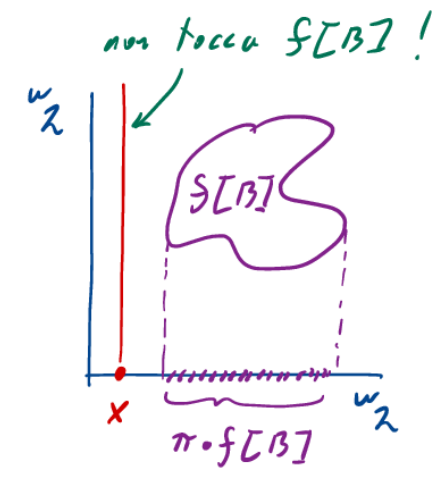
\includegraphics[width = 4cm]{immagini/continuo-numerabile.png}
	\end{figure}
	Quindi, in particolare $\pi \circ f[B] \ne {}^{\omega}2$. Possiamo quindi prendere $x \in {}^{\omega}2 \setminus \pi \circ f[B]$. Dire che $x \not \in \pi \circ f[B]$ significa
	che le coppie con prima componente $x$ nel prodotto sono disgiunte da $f[B]$, cioè $(\underbrace{\{x\} \times {}^{\omega}2}_{= \pi^{-1}(x)}) \cap f[B] = \emptyset$.\\
	E nuovamente, tornando indietro ad $A$ via $f^{-1}$, troviamo $f^{-1}(\{x\} \times {}^{\omega}2) \cap B = \emptyset$, ossia $f^{-1}(\{x\} \times {}^{\omega}2) \subseteq A \setminus B$,
	da cui $|f^{-1}(\{x\} \times {}^{\omega}2)| \leq |A \setminus B|$. Usando il fatto che $f$ è bigettiva:
	\[ |f^{-1}(\{x\} \times {}^{\omega}2)| \overset{\text{$f$ bigett.}}{=} |\{x\} \times {}^{\omega}2| = 1 \cdot 2^{\aleph_0} = 2^{\aleph_0}
		\]
	dunque abbiamo anche la disuguaglianza dal basso e quindi $|A \setminus B| = 2^{\aleph_0}$.
\end{proof}

Siamo finitamente pronti per dimostrare che $|\RR| = 2^{\aleph_0}$.

\begin{proof}(\textcolor{purple}{$|\RR| = 2^{\aleph_0}$})\\
	Siccome $\RR \subseteq \ps(\QQ)$, la disuguaglianza $|\RR| \leq 2^{\aleph_0}$ è immediata. Per dimostrare la disuguaglianza opposta definiamo:
	\[ A \Mydef \{X \in \ps(\omega) | X \ne \emptyset \land |\omega \setminus X| \geq \aleph_0\}
		\]
	ossia i sottoinsiemi di $\omega$ non vuoti e \vocab{coinfiniti}.\\
	\textcolor{MidnightBlue}{\underline{Intuitivamente}: $X \in A$ rappresenta lo sviluppo in notazione binaria di un $x \in\, ]0,1[$ - $x = 0.a_1a_2a_3 \ldots$, $a_i = 1 \leftrightarrow i \in X$ - la condizione $X \ne \emptyset$ serve a escludere lo 0, la 
	condizione di coinfinitezza a escludere l'uno periodico.\footnote{Cioè codificando un sottoinsieme di $\omega$ con una stringa binaria, un insieme che da un certo punto in poi prende tutti i naturali è una stringa binaria con tutti 1 da un certo punto, e quindi il corrispondente numero 0.$a_1a_2\ldots$ ad un certo punto ha un 1 periodico
	\textcolor{MidnightBlue}{- e questa cosa è problematica perché ad esempio $0,1 =  0,011111\ldots$, e ciò fa perdere l'iniettività alla mappa che vogliamo costruire}.
	Tuttavia, imponendo che il sottoinsieme sia coinfinito, abbiamo o che è finito (e quindi da un certo punto in poi c'è 0 definitivamente), oppure è infinito, ma nel contempo ha infiniti punti che non stanno in lui, quindi la stringa non può avere un 1 periodico.}}\\
	Ci basta dimostrare che $|A| = 2^{\aleph_0}$ e che esiste $f : A \rightarrow \RR$ iniettiva. La prima cosa è facile, infatti gli insiemi coinfiniti si ottengono togliendo dalle parti quelli cofiniti (e il vuoto):
	\[ A = \ps(\omega)\setminus (\{\emptyset\} \cup \underbrace{\{X \in \ps(\omega) : |\omega \setminus X|<\aleph_0\}}_{=: S})
		\]
	E l'insieme $S$ dei sottoinsiemi di $\omega$ cofiniti è in corrispondenza biunivoca con $\psf(\omega)$, semplicemente prendendo effettivamente il complementare:
	\[ \ol \square : S \rightarrow \psf(\omega) : X \mapsto \ol X = \omega \setminus X
		\]
	Quindi $|S| = |\psf(\omega)| = \aleph_0$, e, di conseguenza $|A| = |\ps(\omega)\setminus(\{\emptyset\}\cup S)| = 2^{\aleph_0}$, grazie al lemma precedente.
	Resta da costruire $f : A \rightarrow \RR$ iniettiva.\\
	Cominciamo col definire un ordine totale su $A$. Dati $X,Y \in A$ definiamo:
	\[ X <_A Y \Mydef \exists i \in \omega \; \underbrace{(i \cap X = i \cap Y)}_{\forall j \,<\, i \; j \,\in\, X \leftrightarrow j \,\in\, Y} \land \underbrace{(i \in Y \setminus X)}_{i \,\in\, Y\; \land\; i \,\not\in \,X}\,\footnote{Cioè gli elementi più piccoli di $i$ sono nell'intersezione di $X$ e $Y$, per cui $i$ è il più piccolo elemento non comune e $X < Y$ significa che sta in $Y$.}
		\]
	in altri termini, detto $i$ il minimo elemento della differenza simmetrica $X \Delta Y \Mydef (X \setminus Y) \cup (Y \setminus X)$ - che è ben definito perché sono sottoinsiemi di $\omega$ -, se $i \in Y$ - per cui, chiaramente, $i \not \in X$ - allora $X < Y$, se, invece $i \in X$ - per cui $i \not \in Y$ - allora $Y < X$.
	La verifica che un ordine così definito è totale è immediata.\\
	Sia $B \Mydef \psf(\omega) \setminus \{\emptyset\} \subseteq A$, chiaramente $|B| = \aleph_0$, dimostriamo che $B$ è denso in $A$ \textcolor{MidnightBlue}{- cioè i sottoinsiemi finiti di $\omega$ sono densi in quelli coinfiniti}.\\
	Dati $X,Y \in A$, con $X < Y$, e, per definizione, sia $i := \min X \Delta Y$, consideriamo $j := \min \{x \in \omega | x > i \land x \not \in X\}$ - dove l'insieme è non vuoto in quanto $X$ è coinfinito. 
	Ora, dato l'insieme finito $Z := (X \cap j) \cup \{j\}$, verifichiamo che $X < Z < Y$, in questo modo abbiamo che $B$ è denso in $A$.
 	\textcolor{MidnightBlue}{Di fatto, abbiamo mantenuto l'intersezione comune tra $X$ e $Z$ fino a $j$, dopodiché $j \in Z \land j \not \in Z$, per cui $X < Z$. Analogamente, avendo preso $j > i$ e gli stessi elementi di $X$ fino a $j$, accade che $i = \min Z \Delta Y$, per cui $Z < Y$}.
	\begin{figure}[H]
		\centering
		\includegraphics[width = 7.0cm]{immagini/cardinalità_R.png}
	\end{figure}
	Stabilito che $B$ è denso in $A$,  allora, in particolare, $B$ è denso in se stesso, dunque
 	valgono le ipotesi del \hyperref[isoCantor]{isomorfismo di Cantor} e quindi c'è $g : B \rightarrow \QQ$, isomorfismo di ordini.
	Ora, siccome $B$ è denso in $A$, la funzione:
	\[ h : A \rightarrow \; \{\text{sezioni su $B$}\} : X \mapsto B_X = \{Y \in B | Y < X\}
		\]
	è - banalmente ben definita - e iniettiva (perché strettamente crescente). Quindi la mappa $f : A \rightarrow \RR : X \mapsto g[h(X)]$, che prende un insieme coinfinito, lo manda nella sezione di Dedekind da lui generata su $B$,
	e infine nella corrispettiva sezione su $\QQ$, è una funzione - ben posta e - iniettiva da $A$ ad $\RR$, infatti è composizione di due mappe iniettive.
\end{proof}

\subsection{\texorpdfstring{$(\star)$ Alternativa per la cardinalità di $\RR$}{Alternativa per la cardinalità dei reali}}
Vediamo un modo alternativo di stimare dal basso la cardinalità di $\RR$ sfruttando l'insieme di Cantor.
L'idea è che ad successione binaria possiamo associare un punto dell'insieme di Cantor scegliendo semplicemente il percorso sui rami dell'albero della costruzione,
dopodiché - poiché intersechiamo una successione decrescente di compatti - otteniamo un insieme non vuoto da cui prendere il punto di $C$ da far corrispondere alla sequenza binaria.
\begin{figure}[H]
	\centering
	\includegraphics[scale = 0.4]{immagini/cantor-R-cardinalità.png}
\end{figure}
In tal modo avremo $2^{\aleph_0} = |2^{\omega}| \leq |C| \leq |\RR|$.

\begin{proof}
	Definiamo la seguente funzione:
	\[ f : {}^{\omega}2 \to \RR : (a_i)_{i \in \omega} \mapsto \sum_{i = 0}^{\infty} \frac{a_i}{3^i} \;\textcolor{MidnightBlue}{= a_1 \cdot 3^{-1} + a_2 \cdot 3^{-2} + \ldots}
		\]
	\textcolor{MidnightBlue}{- sarebbe una scrittura in base 3 senza la cifra 2\footnote{Potremmo anche fare la stessa cosa buttando
	via 1 anziché 2, ma convenzionalmente si sceglie che è meglio avere 0.1 che 0.0222\ldots. Potremmo altresì usare una base diversa ottenendo la stessa cosa, purché non sia due, in tal caso si procede come la prima dimostrazione vista.}, cioè una cosa del tipo $0.01011100\ldots$,
	dove non abbiamo problemi di ambiguità a causa di periodicità, dati da $0,1 = 0,02222\ldots$, poiché abbiamo tolto il 2 e quindi usiamo solo la prima scrittura. In particolare è come elencare i punti del Cantor fatto in $\left[0,\frac{3}{2}\right]$.}\footnote{Infatti si poteva procedere anche usando il Cantor solito e definendo la mappa da $\{0,2\}^\omega$ a $\RR$,
	che manda una successione in $\sum_{i = 1}^\infty \frac{a_i}{3^i} = \frac 13 \sum_{i = 0}^\infty \frac{a_i}{3^i}$, e in particolare, questa si ottiene dalla funzione precedente moltiplicata per $\frac{2}{3}$ (notare che questa cosa cambia l'insieme numerico da $\{0,1\}$ a $\{0,2\}$ e sistema l'indice per il primo termine della scrittura decimale).}
	\begin{figure}[H]
		\centering
		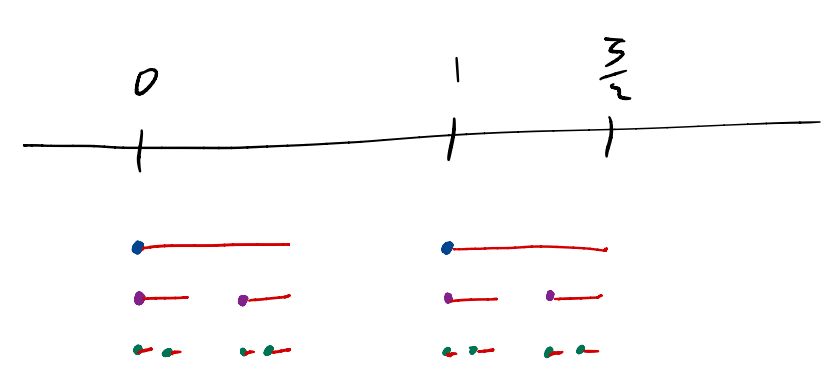
\includegraphics[scale = 0.4]{immagini/cantor_0_32.png}
	\end{figure}
	Dove naturalmente la sommatoria è definita per ricorsione numerabile come funzione da $\omega \to \RR$ nella maniera seguente:
	\[ \sum_{i = 0}^0 \square_i = \square_0 \qquad \sum_{i = 0}^{n + 1} \square_i = \left(\sum_{i = 0}^n \square_i\right) + \square_{n + 1}
		\]
	e la serie è ben definita come:
	\[ \sum_{i = 0}^{\infty}\square_i = \sup_{n \in \omega}\left(\sum_{i = 0}^n \square_i\right)
		\]
	Occorre quindi verificare che $f$ è ben definita ed iniettiva.
	\begin{itemize}
		\item[$\diamondsuit$] \underline{$f$ ben definita}: cioè la serie in arrivo è un elemento di $\RR$, ossia $\sup_{n \in \omega}\left(\sum_{i = 0}^n \frac{a_i}{3}\right)$ esiste,
		e, come sappiamo, ciò è equivalente a chiedere che $\left\{\sum_{i = 0}^n \frac{a_i}{3}\right\}_{n \in \omega}$ ha un maggiorante. Vediamo per induzione che:
		\[ \sum_{i = 0}^n \frac{a_i}{3^i} \leq \frac 32 - \frac{1}{2 \cdot 3^n}
			\]
		fatto questo il RHS si può stimare a sua volta con $\frac 32$ \textcolor{MidnightBlue}{- sarebbe la somma della serie -}, che costituisce un upper bound per ogni $n \in \omega$, quindi per tutti gli elementi dell'insieme.
		\begin{itemize}
			\item[$\boxed{n = 0}$] Banalmente $ \sum_{i = 0}^0 \frac{a_i}{3^i} = \frac{a_0}{3^0} = \frac{a_1}{3} \leq \frac 13 < \frac 43 = \frac 32 - \frac{1}{2 \cdot 3^1}$.
			\item[$\boxed{n \implies n + 1}$] Supponiamo $\sum_{i = 0}^n \frac{a_i}{3^i} \leq \frac 32 - \frac{1}{2 \cdot 3^n}$ e dimostriamo $\sum_{i = 0}^{n+1} \frac{a_i}{3^i} \leq \frac 32 - \frac{1}{2 \cdot 3^{n+1}}$.
			\begin{align*}
				\sum_{i = 0}^{n+1} \frac{a_i}{3^i} &= \left(\sum_{i = 0}^{n} \frac{a_i}{3^i}\right) + \frac{a_{n+1}}{3^{n+1}} &&\text{(def. ricorsiva)} \\
												   &\leq \frac 32 - \frac{1}{2 \cdot 3^n} + \frac{a_{n+1}}{3^{n+1}} &&\text{(hp. induttiva)} \\
												   &\leq \frac 32 - \frac{1}{2 \cdot 3^n} + \frac{1}{3^{n+1}} &&(a_{n+1} \in \{0,1\}) \\
												   &= \frac 32 - \frac{1}{3^n} \cdot \frac 16 = \frac 32 - \frac{1}{2 \cdot 3^{n+1}}
			\end{align*}
		\end{itemize}
		\item[$\diamondsuit$] \underline{$f$ iniettiva}: date due successioni binarie distinte, $(a_i)_{i \in \omega}$ e $(b_i)_{i \in \omega}$, sia $i_0 \in \omega$ il minimo per cui $a_{i_0} \ne b_{i_0}$. Assumiamo WLOG di essere nel caso $a_{i_0} = 0$ e $b_{i_0} = 1$ e 
		verifichiamo che $f(b) > f(a)$ \textcolor{MidnightBlue}{- stiamo proprio verificando la stretta crescenza}. In particolare dimostriamo che:
		\[ f(a) < f(a) + \frac{1}{2 \cdot 3^{i_0}} \leq f(b)
			\]
		Per verificare la seconda disuguaglianza osserviamo che:
		\begin{align*}
			f(a) &= \sup_{n \in \omega} \left(\sum_{i = 0}^n \frac{a_i}{3^i}\right) \\
				 &= \sup_{n \in \omega} \left(\sum_{i < i_0}\frac{a_i}{3^i} + \sum_{i = i_0 + 1}^n \frac{a_i}{3^i} \right) &&(a_{i_0 + 1} = 0) \\
				 &= \sup_{n \in \omega} \left(\sum_{i < i_0}\frac{b_i}{3^i} + \sum_{i = i_0 + 1}^n \frac{a_i}{3^i} \right) &&(\forall i < i_0 \; a_{i} = b_{i}) \\
				 &=\sup_{n \in \omega} \left(\sum_{i < i_0}\frac{b_i}{3^i} + \frac{1}{3^{i_0 + 1}}\sum_{j = 0}^{n - i_0 - 1} \frac{a_{j + i_0 + 1}}{3^j} \right) &&(j = i - i_0 - 1) \\
				 &\leq\sup_{n \in \omega} \left(\sum_{i < i_0}\frac{b_i}{3^i} + \frac{1}{3^{i_0 + 1}} \cdot \frac 32  \right) &&(\text{dalla stima sopra}) \\
				 &= \sum_{i < i_0}\frac{b_i}{3^i} + \frac{1}{2 \cdot 3^{i_0}}  
		\end{align*}
		Ora, dato che:
		\begin{align*}
			f(b) &\geq \sum_{i < i_0}\frac{b_i}{3^i} + \frac{1}{3^{i_0}} \implies \sum_{i < i_0}\frac{b_i}{3^i} \leq f(b) - \frac{1}{3^{i_0}} &&(b_{i_0} = 1)
		\end{align*}
		possiamo concludere la stima sopra:
		\[ f(a) \leq \sum_{i < i_0}\frac{b_i}{3^i} + \frac{1}{2 \cdot 3^{i_0}} \leq f(b) - \frac{1}{3^{i_0}} + \frac{1}{2 \cdot 3^{i_0}} = f(b) - \frac{1}{2 \cdot 3^{i_0}}
			\]
		che è equivalentemente alla seconda disuguaglianza voluta.
	\end{itemize}
\end{proof}

\subsection{\texorpdfstring{$(\star) \; (F,0,1,+,\cdot,\leq)$}{Unicità (a meno di isomorfismo) di un campo ordinato completo}}